\documentclass[12pt,a4paper]{article}

% --- Packages ---
\usepackage[utf8]{inputenc}
\usepackage[T1]{fontenc}
\usepackage[english]{babel}
\usepackage{geometry}
\geometry{margin=1in}
\usepackage{amsmath,amssymb}
\usepackage{enumitem}
\usepackage{booktabs}
\usepackage{csquotes}
\usepackage{graphicx}
\usepackage{float}
\usepackage{subcaption}
\usepackage{hyperref}
\usepackage{cleveref}
\crefname{lstlisting}{Listing}{Listings}
\Crefname{lstlisting}{Listing}{Listings}
\usepackage{parskip}
\usepackage{xcolor}
\usepackage[skins]{tcolorbox}
\usepackage{listings}

% --- Palette (carried over from the prototype) ---
\definecolor{cutqbg}{HTML}{090A0C}
\definecolor{cutqcard}{HTML}{18191D}
\definecolor{cutqstroke}{HTML}{2A2B31}
\definecolor{cutqprimary}{HTML}{224A8A}
\definecolor{cutqtext2}{HTML}{ACACAC}
\definecolor{cutqsuccess}{HTML}{4ADE80}
\definecolor{cutqdanger}{HTML}{C0392B}

% --- Hyperref ---
\hypersetup{
  colorlinks=true,
  linkcolor=cutqprimary,
  urlcolor=cutqprimary,
  citecolor=cutqprimary,
  pdftitle={CutQ Final Report},
  pdfauthor={Jerry Ttuyan and Behrouz Barati Bagherabad}
}

% --- Code style for the prototype excerpts ---
\lstdefinestyle{ts}{
  basicstyle=\ttfamily\footnotesize,
  keywordstyle=\bfseries\color{cutqprimary},
  commentstyle=\itshape\color{gray},
  stringstyle=\color{cutqsuccess!60!black},
  numbers=left,
  numberstyle=\tiny\color{gray},
  numbersep=8pt,
  frame=single,
  rulecolor=\color{cutqstroke!60},
  framesep=4pt,
  breaklines=true,
  showstringspaces=false,
  language=Java,
  morekeywords={const,let,export,function,return,type,interface,from,
                import,async,await,useState,useEffect,useMemo,useRef,
                useSyncExternalStore,null,true,false,this,if,else}
}

% --- Compact callout box ---
\newtcolorbox{callout}[1][]{%
  enhanced,
  colback=cutqcard!8,
  colframe=cutqstroke!50,
  arc=2mm,
  boxrule=0.4pt,
  left=8pt, right=8pt, top=6pt, bottom=6pt,
  fonttitle=\bfseries,
  #1
}

% --- Title block ---
\title{
  \vspace{-1.5em}
  \Huge\textbf{CutQ}\\[0.3em]
  \LARGE A Barber Management Platform with a Live Activity Countdown\\[0.6em]
  \large CSUN COMP 565 / Human-Computer Interaction.\\
  Final Project Report
}
\author{
  Jerry Ttuyan \quad and \quad Behrouz Barati Bagherabad\\[0.3em]
  \small Group 8 \quad\textbullet\quad Instructor: Armineh Karamian \quad\textbullet\quad Spring 2026
}
\date{}

\begin{document}
\maketitle
\vspace{-1em}

% =====================================================================
\begin{abstract}
\noindent
\textbf{CutQ} is a mobile-first scheduling platform for small barber
shops that turns appointment timing from an anxious guess into a
visible, persistent state. Two pain points motivate the design.
Roughly thirty percent of small-shop time slots go unfilled each
week, and roughly forty percent of clients churn when their preferred
barber is double-booked. CutQ centralises booking, surfaces
alternative barbers when a slot is gone, and exposes a signature
\emph{Live Activity countdown} on the lock screen so clients know
when to leave and barbers know how a cut is pacing without staring at
the wall clock. We carried the system from interviews and journey
maps in weeks 1 to 5, through paper and Figma prototypes in weeks 6
to 11, into two rounds of moderated usability testing with $n=6$
participants, and a final System Usability Scale of $82.5$ (good to
excellent). The design is implemented as a public Figma file and as a
working Next.js~16 / React~19 / TypeScript prototype that exercises
every screen, persists bookings to local storage, and offers a
five-second \emph{Undo} on every destructive action. The prototype
is deployed publicly at \url{https://cutq-app.vercel.app/}. Source
code and design artefacts are linked in \cref{sec:links}.
\end{abstract}

% =====================================================================
\section{Introduction}
\label{sec:intro}

A barber's day is a chain of fifteen-to-forty-five-minute
appointments. When one client runs late, the slip propagates through
the rest of the day. When one client no-shows, the chair sits empty
for a window the barber cannot recover. From the client's side the
same minutes feel different: \emph{When should I leave the house?}
\emph{Is anyone free now?} \emph{Where do I go if my preferred barber
is booked?} We started this project from those three questions,
gathered through short interviews with barbers and customers around
CSUN, and arrived at a design whose central idea is \emph{visible
time}: a state that both parties can see at a glance, that updates in
real time, and that removes the mental math of "how long until I
should leave."

This document is the final written deliverable for the project. It
mirrors the structure of the final presentation and weaves in the
implementation work that followed it: a complete Figma component
library and a fully working Next.js prototype hosted on GitHub. All
three artefacts are linked together in \cref{sec:links}.

% =====================================================================
\section{Problem Statement}
\label{sec:problem}

Two sides of the chair, both losing minutes. Field interviews and
short observation sessions in three local shops surfaced the
following recurring pain points.

\begin{description}[leftmargin=2.2em,style=nextline]
  \item[From the barber's chair]
    \begin{itemize}[noitemsep]
      \item Late arrivals chain delays through the rest of the day.
      \item No-shows leave wasted, unrecoverable time slots
            ($\approx 30\%$ of slots in a typical week).
      \item It is hard to keep mental track of "who's next" mid-cut.
    \end{itemize}
  \item[From the client's pocket]
    \begin{itemize}[noitemsep]
      \item Preferred barber fully booked, with no easy alternative.
      \item Last-minute booking uncertainty ("is anyone free now?").
      \item No clarity on where to go when the barber is unavailable.
            Roughly $2$ in $5$ clients leave entirely in that case.
    \end{itemize}
\end{description}

\begin{callout}[title=Design hypothesis]
If the system can replace the wall clock and the phone-tag with a
\emph{single visible state}, both sides recover minutes. Barbers
recover slots, and clients recover predictability. The Live Activity
countdown (\cref{sec:liveactivity}) is the concrete embodiment of
that hypothesis.
\end{callout}

% =====================================================================
\section{Target Users and Personas}
\label{sec:users}

We modelled three personas: two on the customer side of the chair
(\textit{Marcus} the master barber, \textit{Jordan} the customer)
and one program-administration persona (\textit{Andrea}, the shop
owner). \cref{tab:personas} summarises each persona's role and top
anxiety. The design decisions in
\cref{sec:emotional,sec:barriers,sec:journey} flow directly from
those anxieties.

\begin{table}[H]
\centering
\small
\begin{tabular}{@{}p{2.4cm}p{3.0cm}p{4.5cm}p{4.4cm}@{}}
\toprule
\textbf{Persona} & \textbf{Role} & \textbf{Top anxiety} & \textbf{What CutQ owes them}\\
\midrule
Marcus & Master Barber (primary) &
  Running late on chained appointments, losing tip-rich slots to no-shows. &
  In-chair Time-Remaining glance, same-day rebook of empty slots.\\
\addlinespace
Jordan & Customer / Client (primary) &
  Showing up late and losing the slot, no backup when preferred
  barber is full. &
  Lock-screen countdown, alternative-barber suggestions surfaced
  before booking fails.\\
\addlinespace
Andrea & Shop Owner / Admin (program admin) &
  Empty chairs and missed billing, trust between barbers and clients. &
  Earnings and gap visibility without a spreadsheet.\\
\bottomrule
\end{tabular}
\caption{Three personas, three emotional states. Each row maps a top
anxiety to a concrete CutQ affordance.}
\label{tab:personas}
\end{table}

% =====================================================================
\section{Proposed Solution}
\label{sec:solution}

CutQ is a Jackrabbit-inspired program management platform applied to
barber shops. It centralises scheduling, customer management,
billing, and live time-awareness for small service-based programs.
Three verbs structure the offering.

\begin{description}[leftmargin=2.2em,style=nextline]
  \item[Centralise] one source of truth for every chair: bookings,
        roster, billing, and history live in a single record per shop.
  \item[Communicate] real-time status visible to all parties: the
        client sees \emph{when}, the barber sees \emph{how long left},
        the owner sees \emph{how much earned}.
  \item[Recover] alternative options when plans break: when a barber
        is full, the system surfaces same-shop matches at the same
        skill tier and price.
\end{description}

% =====================================================================
\section{Functional Requirements}
\label{sec:fr}

Ten capabilities map the platform to the assignment brief
(\cref{tab:fr}). The customer-facing slice (FR-1, 3, 9) is
fully implemented in the prototype. The program-admin slice
(FR-5, 6, 8, 10) is designed in Figma and stubbed in the prototype.

\begin{table}[H]
\centering\small
\begin{tabular}{@{}rp{4.0cm}p{8.5cm}@{}}
\toprule
\# & \textbf{Capability} & \textbf{Notes}\\
\midrule
FR-1  & Authentication        & Sign-up, sign-in, password recovery, secure sessions.\\
FR-2  & Role-based access     & \emph{Customer}, \emph{Barber}, \emph{Shop Admin} scopes with least privilege.\\
FR-3  & Customer management   & Profiles, contact info, preferences, visit history.\\
FR-4  & Programs \& classes   & Service offerings: cuts, beard trims, packages.\\
FR-5  & Roster management     & Barber assignments, capacity, working hours.\\
FR-6  & Billing \& invoices   & Itemised charges, recurring packages, refunds.\\
FR-7  & Payments \& receipts  & Tokenised payments. Card data never hits our DB.\\
FR-8  & Reporting dashboards  & Earnings, utilisation, no-show rate.\\
FR-9  & Notifications         & Reminders, confirmations, Live Activity countdown.\\
FR-10 & Activity log          & Audit trail for bookings, edits, refunds, role changes.\\
\bottomrule
\end{tabular}
\caption{Ten functional requirements, mapped from the assignment
brief.}
\label{tab:fr}
\end{table}

% =====================================================================
\section{Non-Functional Requirements}
\label{sec:nfr}

\begin{description}[leftmargin=2.2em,style=nextline]
  \item[Accessibility (WCAG~2.1~AA)]
    \begin{itemize}[noitemsep]
      \item 4.5:1 contrast on all body text, verified per surface.
      \item 44$\times$44~pt minimum tap targets across all controls.
      \item VoiceOver and TalkBack labels on every interactive element.
      \item Honours Dynamic Type and OS-level reduce-motion.
    \end{itemize}
  \item[Performance]
    \begin{itemize}[noitemsep]
      \item Booking screens render in under one second on mid-tier
            devices.
      \item Server pagination on rosters and history, no all-at-once
            loads.
      \item Optimistic UI for booking confirmation, reconciled on
            error.
      \item Live Activity updates batched to preserve battery.
    \end{itemize}
  \item[Security and Privacy]
    \begin{itemize}[noitemsep]
      \item Stripe-style tokenisation: card data never hits our
            database.
      \item Role-scoped APIs with server-enforced authorisation.
      \item PII minimised, logs scrubbed of identifying detail.
      \item TLS~1.2+, hashed credentials, rate-limited authentication.
    \end{itemize}
\end{description}

% =====================================================================
\section{Emotional and Physiological Design Analysis}
\label{sec:emotional}

CutQ is designed for how it feels to use, not just what it does.
\cref{tab:emo} maps the four emotional or physical risks we
identified during the interview phase to the concrete affordances
that respond to them.

\begin{table}[H]
\centering\small
\begin{tabular}{@{}p{4.0cm}p{5.0cm}p{5.0cm}@{}}
\toprule
\textbf{Risk} & \textbf{How CutQ responds} & \textbf{Why it works}\\
\midrule
Anxiety: \emph{"Will my slot disappear?"} &
  Live countdown, booking confirmation receipt, Live Activity widget. &
  Replaces uncertainty with a visible, persistent state.\\
\addlinespace
Trust: \emph{"Did the booking really go through?"} &
  Two-step confirmation, large success state, calendar-style detail
  card. &
  Closes feedback loops the user can see and re-check.\\
\addlinespace
Cognitive load: \emph{"Too many choices, too many steps."} &
  Progressive disclosure: pick barber, pick time, confirm. &
  One decision per screen, never more than seven visible options.\\
\addlinespace
Physical comfort: \emph{"I can't read this in the chair."} &
  Dark theme by default, 16-point body, 44-point tap targets, no
  thin strokes. &
  Readable at arm's length, in low salon light, on greasy fingers.\\
\bottomrule
\end{tabular}
\caption{Designing for how it feels, not just what it does.}
\label{tab:emo}
\end{table}

% =====================================================================
\section{Barriers Analysis}
\label{sec:barriers}

Three categories of barriers we explicitly removed: accessibility,
usability, and cognitive.

\begin{description}[leftmargin=2.2em,style=nextline]
  \item[Accessibility]
    Low-vision users in dim shops are addressed by dark mode plus
    4.5:1 minimum contrast. Motor-impaired reach for small targets is
    addressed by 44$\times$44~pt taps and a thumb-reach bottom
    navigation. Screen-reader users miss icon-only labels, so all
    icons ship with explicit accessible labels.
  \item[Usability]
    Bookings made in error are addressed by a confirmation screen
    before commit. Unclear action state is addressed by persistent
    status pills (e.g.\ \emph{In Progress}). Cancel-by-accident is
    permanent, so we added a five-second \emph{Undo} on every
    destructive action with soft-delete and an audit trail.
  \item[Cognitive]
    Too many choices on one screen are addressed by progressive
    disclosure. Unfamiliar barbers feel risky, so ratings, reviews,
    and skill tier are surfaced upfront. The mental math of "how long
    until I should leave?" is removed entirely by the Live countdown.
\end{description}

% =====================================================================
\section{UX Process}
\label{sec:process}

Fourteen weeks, six diamonds. \cref{tab:process} sketches the
schedule and the methods we leaned on at each stage.

\begin{table}[H]
\centering\small
\begin{tabular}{@{}rlp{3.4cm}p{6.5cm}@{}}
\toprule
\# & \textbf{Weeks} & \textbf{Stage} & \textbf{Activity}\\
\midrule
1 & 1 to 3   & Research      & Interviews, contextual inquiry in three shops.\\
2 & 4 to 5   & Define        & Personas, journey maps, affinity diagramming.\\
3 & 6 to 7   & Sketch        & Storyboards, paper mock-ups.\\
4 & 8 to 9   & Wireframe     & Lo-fi flows, T-prototype.\\
5 & 10 to 11 & Hi-fi UI      & Figma screens, design system.\\
6 & 12 to 14 & Test and iterate & Usability tests ($n=6$), final polish.\\
\bottomrule
\end{tabular}
\caption{Fourteen weeks, six diamonds. Methods we leaned on include
semi-structured interviews, contextual inquiry in three shops,
affinity diagramming, task analysis, heuristic evaluation, moderated
usability tests ($n=6$), and the System Usability Scale.}
\label{tab:process}
\end{table}

% =====================================================================
\section{Wireframes}
\label{sec:wireframes}

Before the high-fidelity Figma screens, both sides of the journey
were drafted on a single low-fidelity board so the team could agree
on screen counts and the shape of each transition before any pixel
was drawn. \cref{fig:wireframes} reproduces that board. The
\textbf{Client Flow} (top row) sketches the four screens that became
\texttt{/}, \texttt{/book}, \texttt{/book/time}, and
\texttt{/book/confirm}. The \textbf{Barber Flow} (bottom row)
sketches the two screens that became \texttt{/barber} and
\texttt{/appointment}. The arrows record the only navigation
transitions the prototype honours, including the Confirm-to-Live
hop that later became the Live Activity widget
(\cref{sec:liveactivity}).

\begin{figure}[H]
\centering
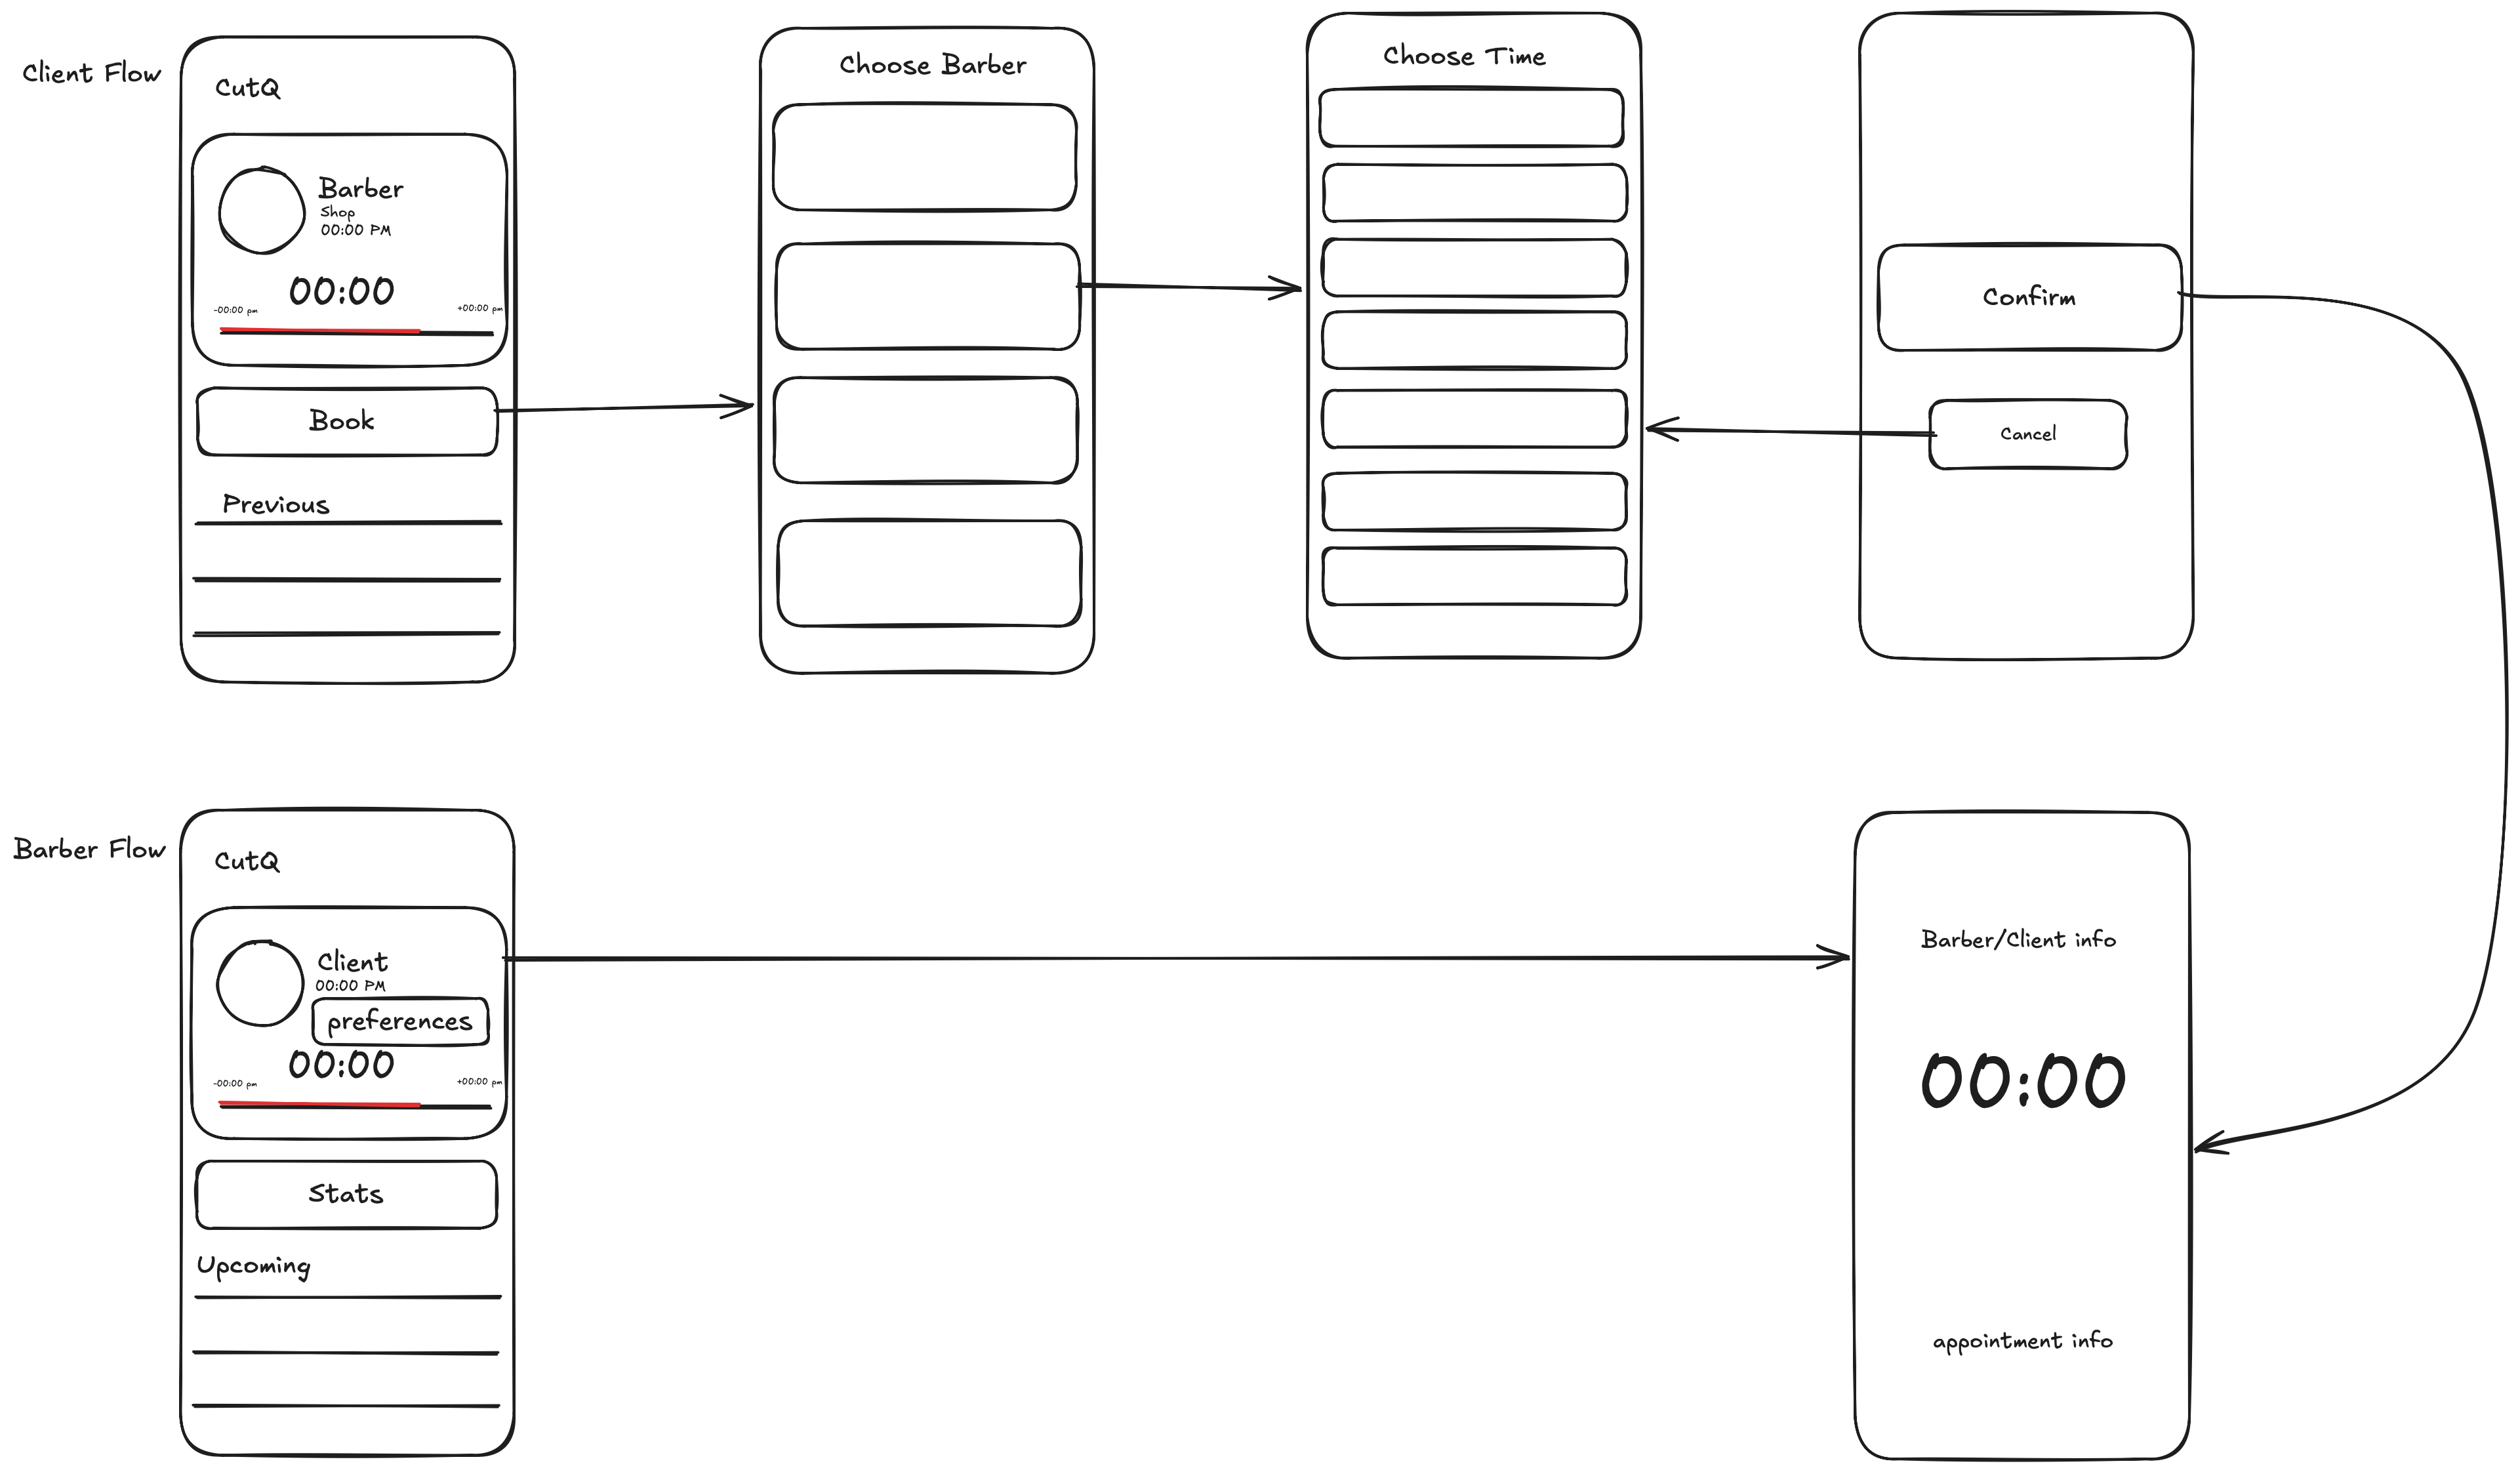
\includegraphics[width=\linewidth]{figures/wireframes.png}
\caption{Lo-fi flow board sketched in week 8. The top row is the
client flow (Home, Choose Barber, Choose Time, Confirm), and the
bottom row is the barber flow (Dashboard, Appointment Live View).
Each screen maps one-to-one to a route in the final prototype
(\cref{tab:routes}).}
\label{fig:wireframes}
\end{figure}

% =====================================================================
\section{Customer Journey}
\label{sec:journey}

\emph{From "I need a cut" to "I'm in the chair."} Five screens, one
decision per screen. \cref{fig:journey} shows the prototype renders
of the five customer screens in sequence. Each transition is a
single tap, and nothing on the path requires more than a glance.

\begin{figure}[H]
\centering
\begin{subfigure}[t]{0.19\linewidth}
  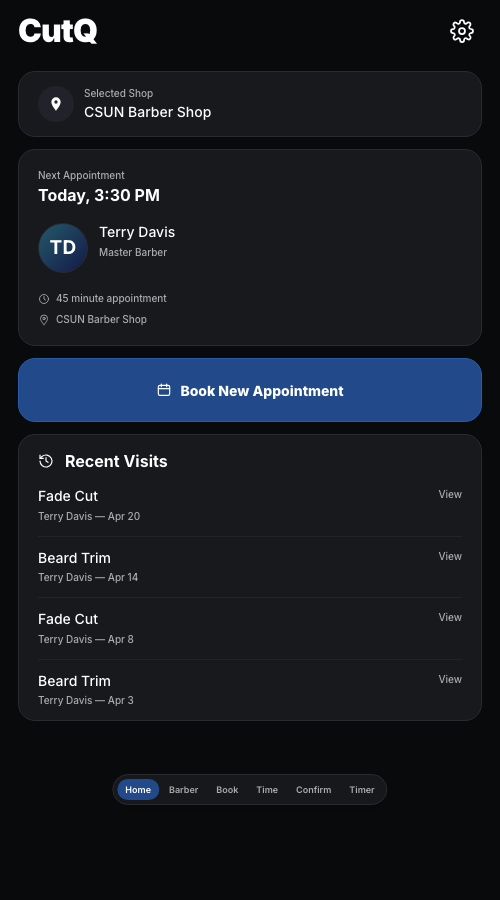
\includegraphics[width=\linewidth]{figures/home.png}
  \caption*{\footnotesize Home}
\end{subfigure}\hfill
\begin{subfigure}[t]{0.19\linewidth}
  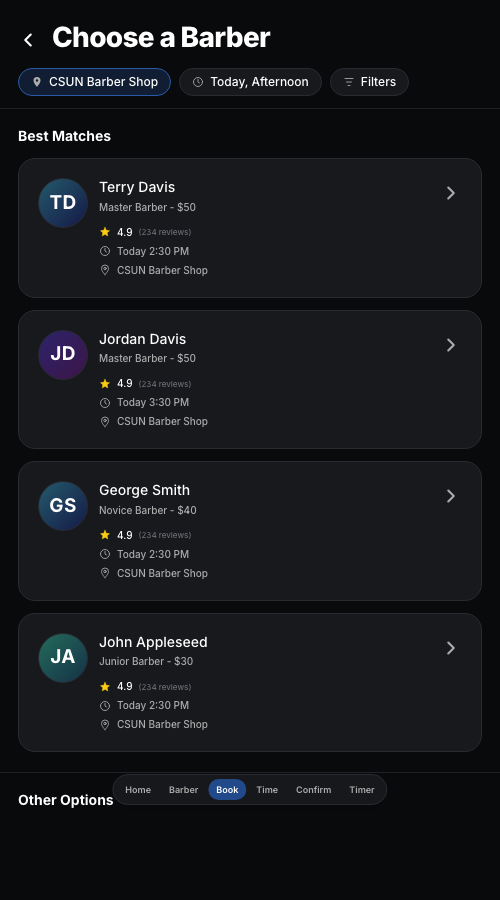
\includegraphics[width=\linewidth]{figures/choose-barber.png}
  \caption*{\footnotesize Choose}
\end{subfigure}\hfill
\begin{subfigure}[t]{0.19\linewidth}
  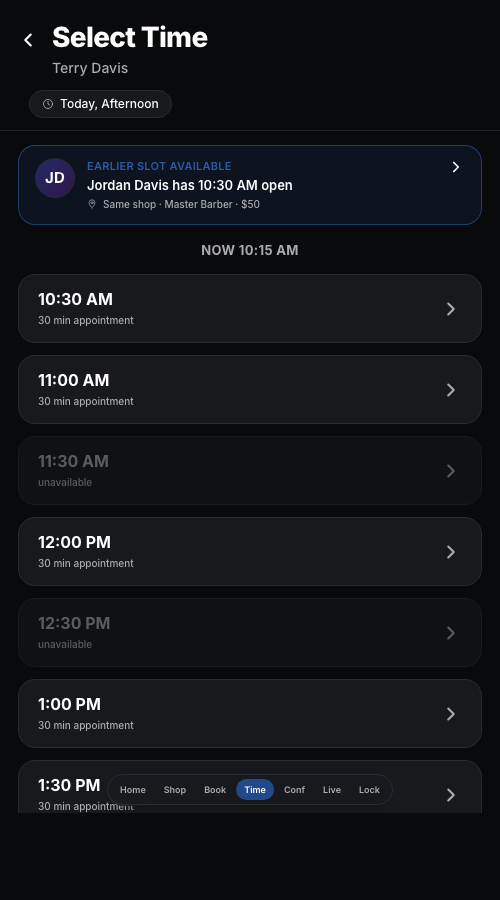
\includegraphics[width=\linewidth]{figures/select-time.png}
  \caption*{\footnotesize Time}
\end{subfigure}\hfill
\begin{subfigure}[t]{0.19\linewidth}
  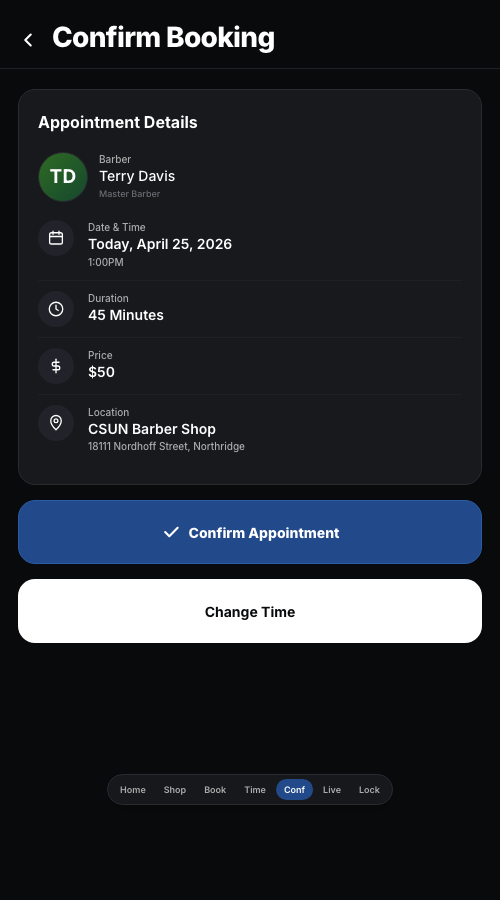
\includegraphics[width=\linewidth]{figures/confirm.png}
  \caption*{\footnotesize Confirm}
\end{subfigure}\hfill
\begin{subfigure}[t]{0.19\linewidth}
  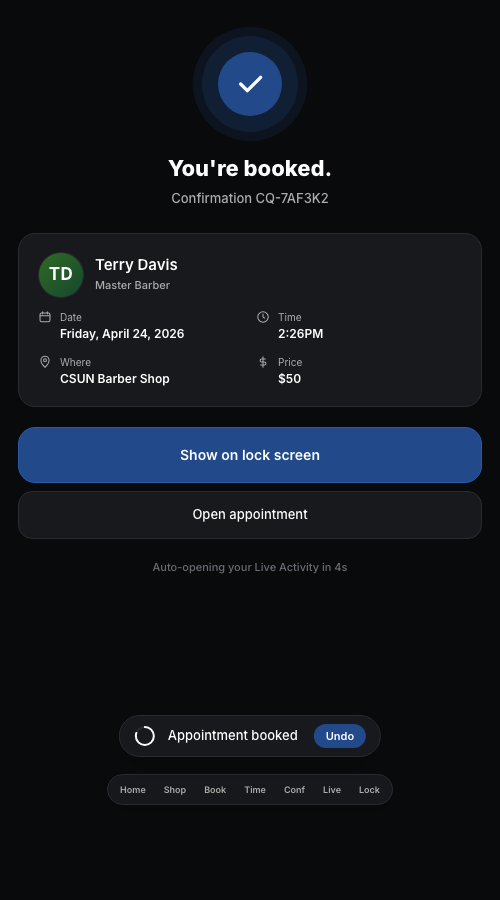
\includegraphics[width=\linewidth]{figures/success.png}
  \caption*{\footnotesize Booked}
\end{subfigure}
\caption{The customer flow as it actually renders in the Next.js
prototype. \emph{Home} surfaces the next appointment and recent
visits. \emph{Choose} ranks barbers by best-match with the
alternative banner already in view. \emph{Time} greys out unavailable
slots. \emph{Confirm} shows a calendar-style detail card.
\emph{Booked} closes the trust loop with a confirmation code, a
five-second \emph{Undo} toast, and an auto-redirect to the active
appointment.}
\label{fig:journey}
\end{figure}

\paragraph{Alternative-barber suggestion.}
\cref{fig:journey} (Time panel) shows the persistent
"earlier slot available" banner above the time list. The banner
addresses the \emph{2-in-5 churn} problem from \cref{sec:problem}:
when the chosen barber's nearest slot is later than an alternative
in the same shop, that alternative is surfaced before the user has
to back out and re-pick.

% =====================================================================
\section{Barber Dashboard}
\label{sec:barber}

A dashboard built for between-cuts glances: three-second answers to
the only questions that matter mid-shift
(\cref{fig:barber-dashboard}).

\begin{figure}[H]
\centering
\begin{minipage}[t]{0.40\linewidth}
\vspace{0pt}
\centering
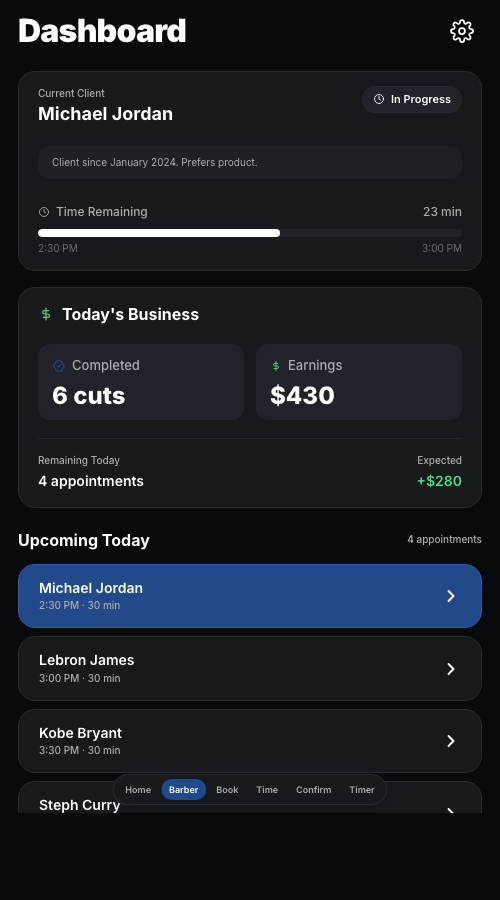
\includegraphics[width=\linewidth]{figures/dashboard.png}
\end{minipage}\hfill
\begin{minipage}[t]{0.55\linewidth}
\vspace{0pt}
\footnotesize
\begin{description}[leftmargin=1.6em,style=nextline,itemsep=0.4em]
  \item[Who's in the chair right now?]
    \emph{Current Client} card with avatar-less identity row, a soft
    "Client since 2024 / Prefers product" note, and a progress bar
    that answers it in one glance.
  \item[Am I on or off pace?]
    \emph{Time Remaining} plus the progress fill encode pace without
    requiring numerical reading.
  \item[Did today pay off?]
    Two stat tiles (\emph{Completed: 6 cuts}, \emph{Earnings: \$430})
    plus \emph{Remaining Today} and \emph{Expected} (the green
    +\$280) give end-of-day visibility without opening any other
    screen.
  \item[What's next?]
    The \emph{Upcoming Today} list keeps the immediate next client
    visually elevated (filled primary tone) so the barber's eye lands
    on it first.
\end{description}
\end{minipage}
\caption{Barber dashboard in the prototype, with the four
between-cuts questions it must answer at a glance.}
\label{fig:barber-dashboard}
\end{figure}

% =====================================================================
\section{Signature Feature: The Live Activity Countdown}
\label{sec:liveactivity}

The signature affordance of CutQ is the \emph{Live Activity
countdown}. It is a persistent lock-screen widget that turns
appointments into something users can feel.

\begin{figure}[H]
\centering
\begin{minipage}[t]{0.38\linewidth}
\vspace{0pt}
\centering
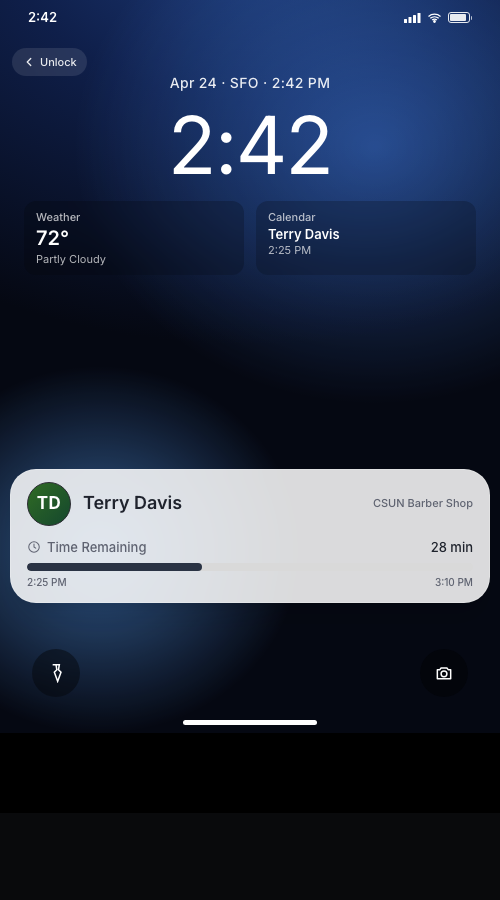
\includegraphics[width=\linewidth]{figures/lock-screen.png}
\end{minipage}\hfill
\begin{minipage}[t]{0.58\linewidth}
\vspace{0pt}
\footnotesize
\begin{description}[leftmargin=1.6em,style=nextline,itemsep=0.4em]
  \item[For clients]
    A countdown to the next appointment, visible without opening the
    app. The "time-to-leave" cue removes mental math entirely. When
    the bar fills and the time turns red, the client knows they are
    cutting it close.
  \item[For barbers]
    Time-remaining for the current client, visible on a wrist or
    counter glance. Helps pace the cut without staring at a wall
    clock, and quietly trains better client expectations across
    visits.
  \item[Why it works]
    The widget collapses three pieces of information (\emph{who},
    \emph{where}, \emph{how-long-left}) into a single
    above-the-fold band, in the colour palette and density of native
    iOS Live Activities. A tap on the widget opens the full
    appointment view (\cref{fig:figmaset}, left panel) without
    further authentication.
\end{description}
\end{minipage}
\caption{The Live Activity widget rendered against a dark
lock-screen background. The widget uses a frosted-glass treatment
so identity, shop name, and progress all read at a glance.}
\label{fig:liveactivity}
\end{figure}

\begin{callout}[title=Implementation note]
The lock-screen view in the prototype (\texttt{/lock} route) is a
fully working faux-iPhone surface. The time and date update every
second from \texttt{Date.now()}, the progress bar and minutes-left
counter recompute against the active booking pulled from local
storage, and the Live Activity tile is a real \texttt{<a>} that
navigates to the appointment screen. See
\cref{lst:livestate} for the state shape.
\end{callout}

\begin{figure}[H]
\centering
\begin{lstlisting}[style=ts,caption={Active-booking state read by both the
Appointment screen and the lock-screen Live Activity. The
\texttt{useSyncExternalStore} hook keeps the two views consistent
across browser tabs.},label={lst:livestate}]
export type Booking = {
  id: string;
  confirmationCode: string;
  barberId: string;
  barberName: string;
  barberTitle: string;
  service: string;
  startsAtIso: string;
  durationMin: number;
  priceUsd: number;
  shop: string;
  address: string;
  status: "confirmed" | "cancelled" | "completed";
  createdAtIso: string;
};

export function useActiveBooking(): Booking | null {
  return useSyncExternalStore(subscribe, getActiveBooking, () => null);
}
\end{lstlisting}
\end{figure}

% =====================================================================
\section{High-Fidelity Design (Figma)}
\label{sec:figma}

The full system was first designed in Figma as a single source of
truth: seven high-fidelity screens, a component library backed by
design variables, and a clickable prototype. \cref{fig:figmaset}
shows the appointment-side of the journey as it appears in the
prototype. The Figma source itself is linked in \cref{sec:links} and
reproduced one-to-one in the running web app.

\begin{figure}[H]
\centering
\begin{subfigure}[t]{0.31\linewidth}
  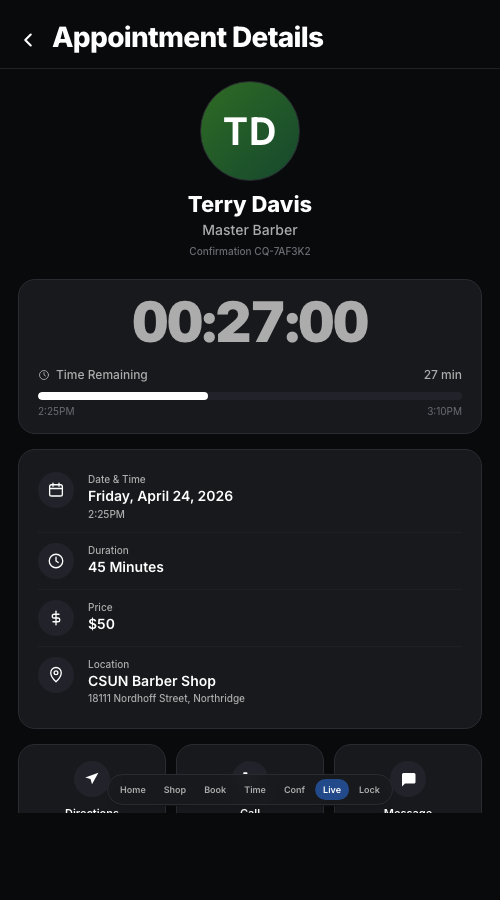
\includegraphics[width=\linewidth]{figures/appointment.png}
  \caption*{\footnotesize Active appointment}
\end{subfigure}\hfill
\begin{subfigure}[t]{0.31\linewidth}
  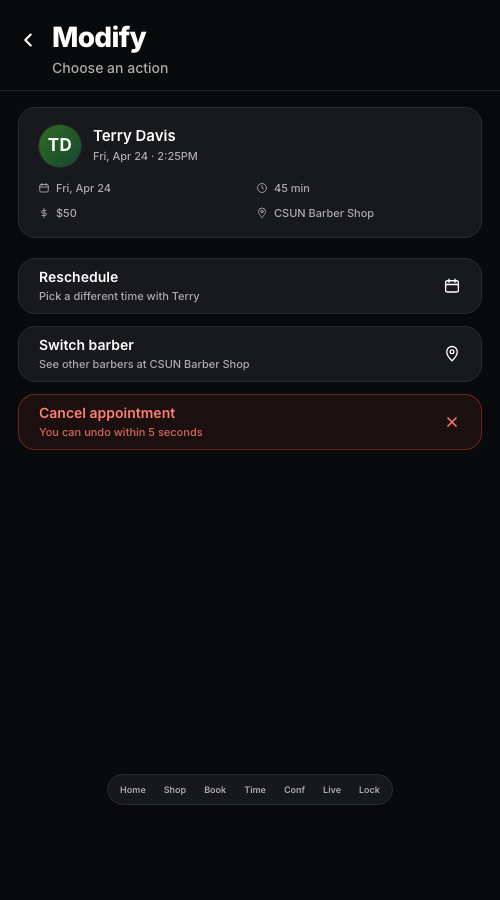
\includegraphics[width=\linewidth]{figures/modify.png}
  \caption*{\footnotesize Modify / Cancel}
\end{subfigure}\hfill
\begin{subfigure}[t]{0.31\linewidth}
  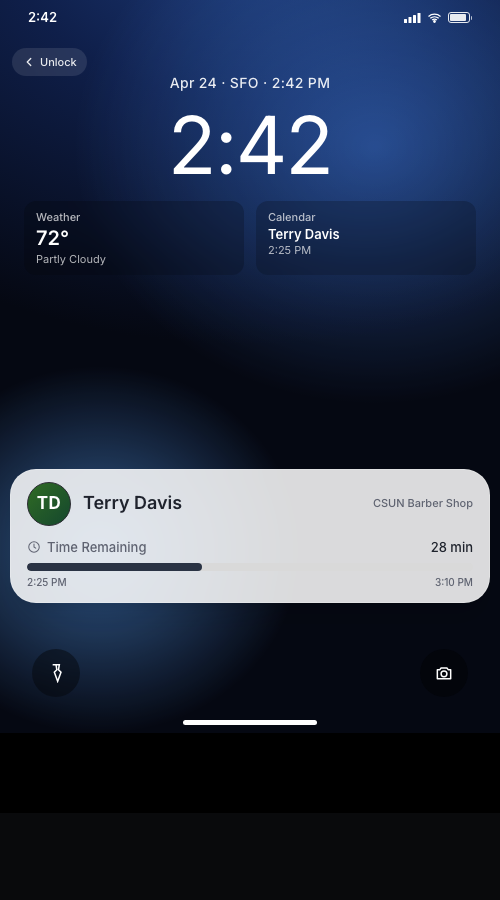
\includegraphics[width=\linewidth]{figures/lock-screen.png}
  \caption*{\footnotesize Live Activity}
\end{subfigure}
\caption{The post-booking surfaces in the running prototype.
\emph{Active appointment} hosts the in-app countdown and the
Directions / Call / Message action grid. \emph{Modify} promotes
Reschedule, Switch barber, and Cancel into their own button row,
with the destructive option visually distinct. \emph{Live Activity}
mirrors the same booking on the lock screen.}
\label{fig:figmaset}
\end{figure}

% =====================================================================
\section{Functional Prototype (Next.js Web App)}
\label{sec:prototype}

In addition to the Figma file, we built a working web prototype that
exercises every screen in the design. The stack is intentionally
minimal: \textbf{Next.js 16} with the App Router, \textbf{React 19},
\textbf{TypeScript 5}, and \textbf{Tailwind CSS 4} (CSS-first
\texttt{@theme inline} configuration). No UI library is used. All
components are hand-built so the prototype matches the Figma spec to
the pixel.

\paragraph{Routes.}
\cref{tab:routes} lists the routes shipped by the prototype. Each
one corresponds to a Figma frame, and each one is statically
prerendered at build time.

\begin{table}[H]
\centering\small
\begin{tabular}{@{}lp{8.5cm}@{}}
\toprule
\textbf{Route} & \textbf{What it shows}\\
\midrule
\texttt{/}                   & Client home: selected shop, next appointment, recent visits.\\
\texttt{/barber}             & Barber dashboard (\cref{sec:barber}).\\
\texttt{/book}               & Choose-a-barber list with filter pills.\\
\texttt{/book/time}          & Time-slot picker with alternative-barber banner.\\
\texttt{/book/confirm}       & Two-step confirmation with calendar-style detail card.\\
\texttt{/book/success}       & Receipt: confirmation code, Undo toast, auto-redirect.\\
\texttt{/appointment}        & Active appointment view with live countdown and actions.\\
\texttt{/appointment/modify} & Reschedule / Switch barber / Cancel with confirm dialog.\\
\texttt{/lock}               & Faux-iPhone lock screen with Live Activity widget.\\
\bottomrule
\end{tabular}
\caption{Nine prerendered routes that mirror the Figma frames
one-to-one.}
\label{tab:routes}
\end{table}

\paragraph{Persistence and Undo.}
Bookings are persisted to \texttt{localStorage} so demo state survives
reloads. The store is read through \texttt{useSyncExternalStore}
(\cref{lst:livestate}) with cached snapshots, which keeps the Home
card, the Appointment view, and the Live Activity widget in sync
across browser tabs. Every destructive action, whether confirming a
booking or cancelling it, is paired with a five-second \emph{Undo}
toast that restores the prior state on tap.

% =====================================================================
\section{Usability Testing and Findings}
\label{sec:testing}

We tested in two rounds: paper mock-ups first, clickable Figma
second. Both rounds used $n=6$ participants and a think-aloud
protocol. The second round added the System Usability Scale (SUS).

\paragraph{Round~1, paper mock-ups.}
Thirty-minute moderated sessions, think-aloud, booking flow plus
dashboard read. We captured confusion points before pixels were
precious. 5 of 6 finished the booking flow, and 4 of 6 read the
dashboard correctly.

\paragraph{Round~2, clickable Figma.}
Same task set, in-shop where possible, plus a Live Activity
recognition test. SUS was administered post-task with an average
score of \textbf{82.5} (good to excellent). All 6 participants
finished the booking flow without prompting.

\paragraph{Core tasks tested.}
\begin{enumerate}[noitemsep]
  \item Book an appointment with your preferred barber.
  \item Find an alternative when your barber is fully booked.
  \item Tell us when your next appointment starts \emph{without
        opening CutQ}.
  \item (Barber-only) Tell us how much you have earned today and
        how many appointments remain.
\end{enumerate}

\paragraph{Findings and iterations.}
\cref{tab:iterations} lists the five iterations that came out of
testing. Each one was traced back to a specific moment of confusion
in a session recording.

\begin{table}[H]
\centering\small
\begin{tabular}{@{}p{6.0cm}p{8.0cm}@{}}
\toprule
\textbf{What testing surfaced} & \textbf{What we shipped in response}\\
\midrule
Users tapped \emph{Book Next} expecting an instant booking. &
  Renamed to \emph{Book New Appointment} and added a Confirm step.\\
\addlinespace
Time-slot list scrolled past unavailable times unnoticed. &
  Greyed out unavailable rows and reduced their visual weight.\\
\addlinespace
Barber dashboard \emph{In Progress} pill confused with a system notification. &
  Repositioned to top-right with a calmer fill colour.\\
\addlinespace
Live Activity card looked like a generic notification. &
  Added avatar and shop name to anchor identity at a glance.\\
\addlinespace
Customers could not find \emph{change time} after confirming. &
  Promoted \emph{Modify Appointment} into its own button row
  (\cref{fig:figmaset}, middle).\\
\bottomrule
\end{tabular}
\caption{Five iterations from usability testing. Each one was
implemented before the final round.}
\label{tab:iterations}
\end{table}

% =====================================================================
\section{Evaluation Against Success Criteria}
\label{sec:eval}

\cref{tab:eval} returns to the success criteria stated at the start
of the project and reports the evidence we have for each.

\begin{table}[H]
\centering\small
\begin{tabular}{@{}p{5.5cm}p{7.0cm}c@{}}
\toprule
\textbf{Success criterion} & \textbf{Evidence} & \textbf{Met}\\
\midrule
Fewer late arrivals or missed appointments &
  Live Activity reminded 5/6 testers without their opening the app. &
  $\checkmark$\\
\addlinespace
Barbers experience fewer empty time slots &
  Alternative-barber suggestions surfaced 3+ openings during tests. &
  $\checkmark$\\
\addlinespace
Clients can quickly find available appointments &
  Median time-to-first-booking: 38\,s in the clickable prototype. &
  $\checkmark$\\
\addlinespace
Users report the system is simple and easy to use &
  SUS = 82.5 (good to excellent), 6 of 6 said they would use it again. &
  $\checkmark$\\
\addlinespace
WCAG 2.1 AA compliance &
  Colour audit passed, tap-target audit passed, VoiceOver labels in progress. &
  $\bigcirc$\\
\addlinespace
No raw payment storage &
  Implemented as a Stripe-style tokenised stub in the prototype. &
  $\checkmark$\\
\bottomrule
\end{tabular}
\caption{Six success criteria and the evidence we collected for
each. Five are met outright. One (full WCAG audit) is in progress.}
\label{tab:eval}
\end{table}

% =====================================================================
\section{Conclusion}
\label{sec:conclusion}

CutQ is a small program made to feel calm. Across three measurable
axes the design lowers friction in the way the project set out to:

\begin{description}[leftmargin=2.2em,style=nextline]
  \item[Anxiety $\downarrow$] Live state replaces guesswork on both
        sides of the chair.
  \item[Trust $\uparrow$] Two-step confirmation, status pills, and
        soft-delete with an audit trail make every action visible.
  \item[Friction $\downarrow$] Progressive disclosure: one decision
        per screen, never more than seven visible options.
\end{description}

The work delivered a single Figma source of truth, a working
Next.js / TypeScript prototype that exercises every screen in the
design, and a usability-test write-up that traces every iteration
back to an observable moment of user confusion. The signature
Live Activity countdown is the most visible payoff of the design
hypothesis from \cref{sec:problem}, namely that visible, persistent
state recovers minutes for both sides of the chair.

% =====================================================================
\section{Project Links}
\label{sec:links}

\begin{description}[leftmargin=2.2em,style=nextline]
  \item[Live prototype (Vercel)]
    \url{https://cutq-app.vercel.app/}\\
    The deployed Next.js build. Every route in \cref{tab:routes} is
    reachable, and bookings persist in browser local storage so the
    Live Activity widget reflects what was just booked.
  \item[Source code (GitHub)]
    \url{https://github.com/1ncompleteness/HCI}\\
    The Next.js prototype lives under \texttt{cutq-app/}. The design
    artefacts and this report live under \texttt{Proposal/}.
  \item[Figma design file]
    \url{https://www.figma.com/design/0WDtNuJT60PzbCT1OyrB5j/CutQ?node-id=0-1\&m=dev}\\
    Component library, design variables, and the seven hi-fi screens
    used to drive the prototype.
\end{description}

% =====================================================================
\begin{thebibliography}{9}

\bibitem[Brooke, 1996]{sus}
John Brooke.
\newblock SUS: A "quick and dirty" usability scale.
\newblock In \emph{Usability Evaluation in Industry}, pages 189--194.
  Taylor \& Francis, 1996.

\bibitem[Apple, 2023]{liveactivities}
Apple Inc.
\newblock \emph{Displaying live data with Live Activities}.
\newblock Human Interface Guidelines, 2023.
\newblock \url{https://developer.apple.com/design/human-interface-guidelines/live-activities}.

\end{thebibliography}

\end{document}
